
\section{Tafel ronde 1: Slimste mens}
Freddy doet mee met de slimste mens, help jij hem?
geef de naam van de persoon waarop freddy is geplakt

\begin{questions}

\question[2] {
\begin{center}
{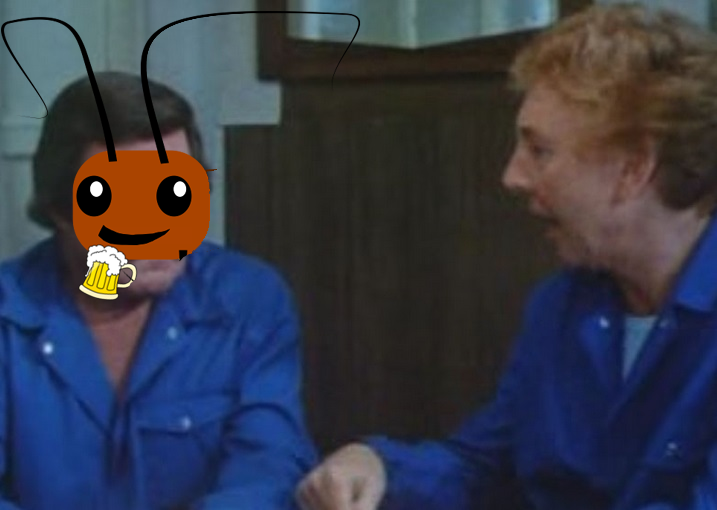
\includegraphics[scale=0.40]{1}}
\end{center}
\begin{flushleft}
\makebox[\textwidth]{Volledige naam: Gaston Berghmans }
\end{flushleft} }
\question[2] {
\begin{center}
{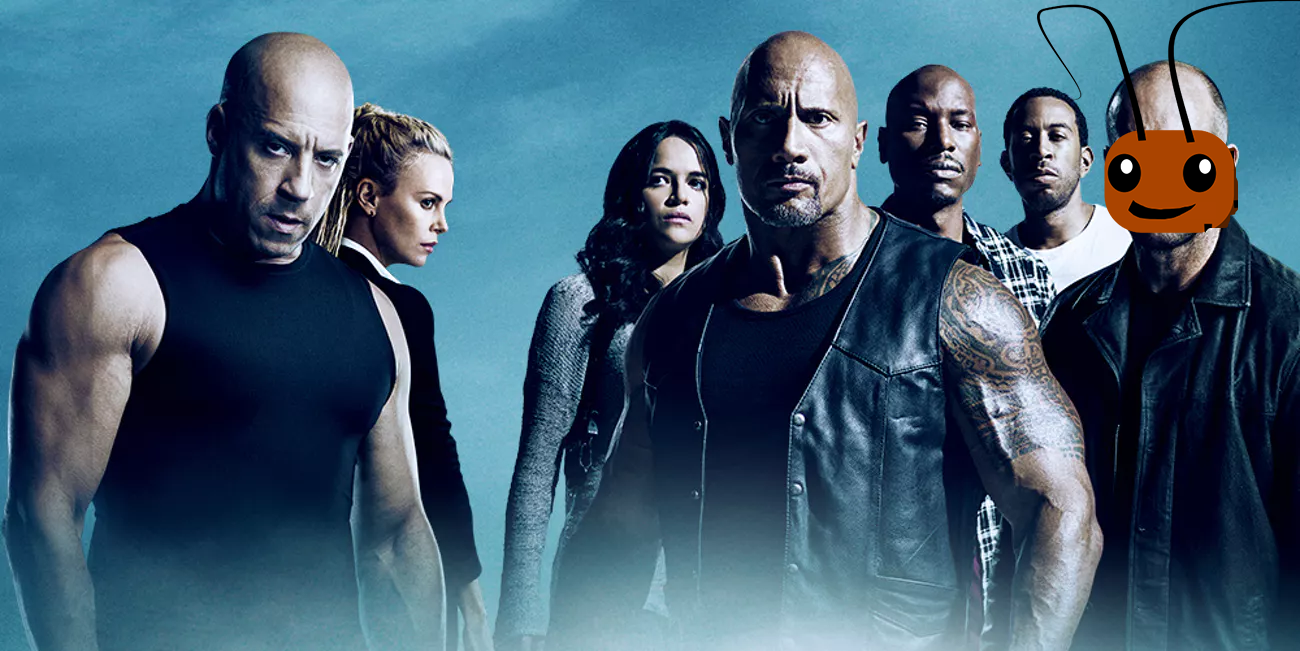
\includegraphics[scale=0.20]{2}}
\end{center}
\begin{flushleft}
\makebox[\textwidth]{naam:Luc Turlinckx / Ben Segers }
\end{flushleft} }
\question[1] {
\begin{center}
{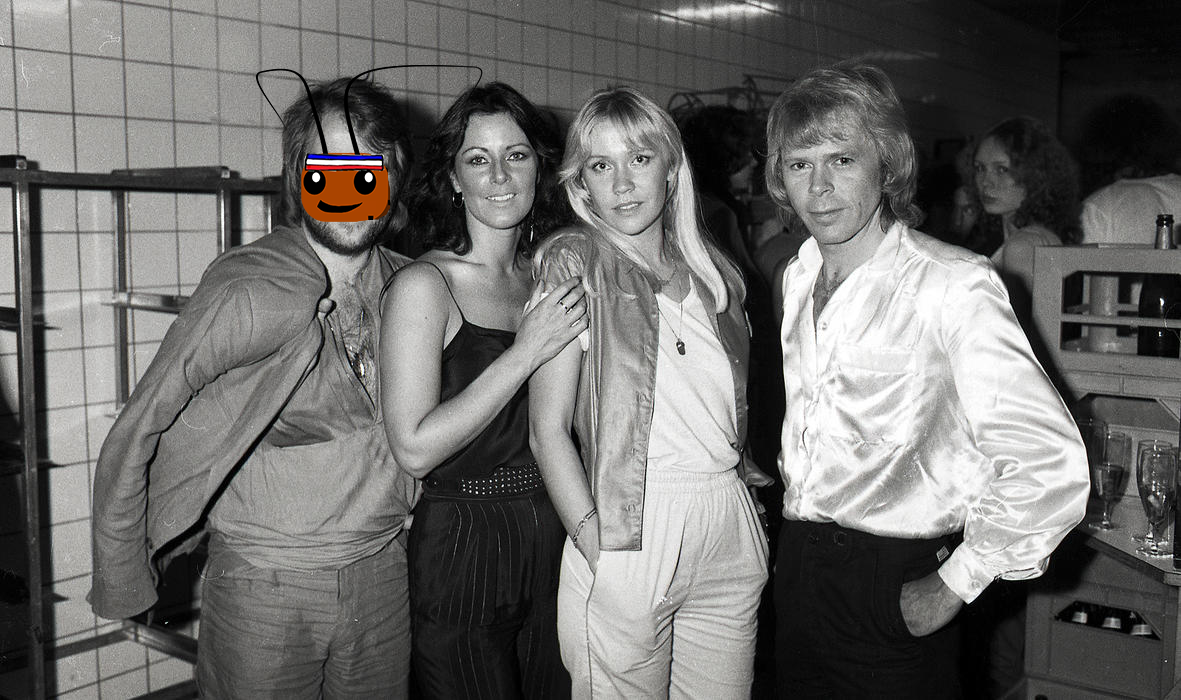
\includegraphics[scale=0.30]{3}}
\end{center}
\begin{flushleft}
\makebox[\textwidth]{naam:Meowth}
\end{flushleft} }
\question[1] {
\begin{center}
{
\includegraphics[scale=0.15]{4}}
\end{center}
\begin{flushleft}
\makebox[\textwidth]{naam:Deckard Shaw / Jason Statham }
\end{flushleft} }
\question[1] {
\begin{center}
{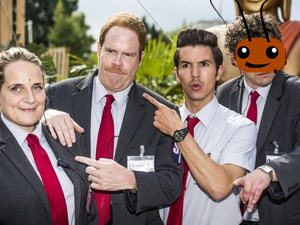
\includegraphics[scale=0.80]{5}}
\end{center}
\begin{flushleft}
\makebox[\textwidth]{naam: Benny Andersson }
\end{flushleft} }

\question[3]{
{
\begin{table}[h]
\centering
\begin{tabular}{llll}
\textbf{Amerikaan} & \textbf{Verbranding}          & \textbf{Rapper} & \textbf{Nummer}    \\
\textbf{Zweepslag}      & \textbf{Van voor naar achter} & \textbf{Acteur}       & \textbf{Genie in Aladdin }   \\
\textbf{Auschwitz} & \textbf{Letsel}           & \textbf{Joden}          & \textbf{Nek}
\end{tabular}
\end{table}
}
\begin{flushleft}
\makebox[\textwidth]{Link 1: Lance armstrong\linebreak}
\makebox[\textwidth]{Link 2:noodnummers}
\makebox[\textwidth]{Link 3:Slag om het gravensteen}
\end{flushleft}
}

\question[3]{
{\begin{table}[h]
\centering
\begin{tabular}{llll}
\textbf{VTM} & \textbf{Citroen}          & \textbf{Brussel} & \textbf{Sunrise}    \\
\textbf{CSI}      & \textbf{Parijs} & \textbf{Mexicaans}       & \textbf{The Simpsons}   \\
\textbf{London} & \textbf{Zout}           & \textbf{Amsterdam}          & \textbf{Temptation Island }
\end{tabular}
\end{table}
}
\begin{flushleft}
\makebox[\textwidth]{Link 1:Will smith}
\makebox[\textwidth]{Link 2:Concentratiekampen}
\makebox[\textwidth]{Link 3:Whiplasch}
\end{flushleft}
}

\question[3]{
{\begin{table}[h]
\centering
\begin{tabular}{llll}
\textbf{Bieten} & \textbf{Klein}          & \textbf{De pil} & \textbf{Condoom}    \\
\textbf{Kristalstructuur}      & \textbf{Spielberg} & \textbf{Pessarium}       & \textbf{Telefoneren}   \\
\textbf{Riet} & \textbf{Buitenaards}           & \textbf{CH20}          & \textbf{Spiraaltje}
\end{tabular}
\end{table}
}
\begin{flushleft}
\makebox[\textwidth]{Link 1:Tequilla}
\makebox[\textwidth]{Link 2:Hoofdsteden}
\makebox[\textwidth]{Link 3:Tv-programma's}
\end{flushleft}
}
\newpage
\question[3]{
{\begin{table}[h]
\centering
\begin{tabular}{llll}
\textbf{Dagboek} & \textbf{Papier}          & \textbf{Joods meisje} & \textbf{Bezem}    \\
\textbf{Onderduiken}      & \textbf{Kraanvogel} & \textbf{Brandstapel}       & \textbf{Japans}   \\
\textbf{Vouwen} & \textbf{vrouw}           & \textbf{Schuilhuis}          & \textbf{Neuswrat}
\end{tabular}
\end{table}
}
\begin{flushleft}
\makebox[\textwidth]{Link 1:suiker}
\makebox[\textwidth]{Link 2:Voorbehoedsmiddel}
\makebox[\textwidth]{Link 3:E.T.}
\end{flushleft}
}
\question[3]{
{\begin{table}[h]
\centering
\begin{tabular}{llll}
\textbf{Neuswrat} & \textbf{rapper}          & \textbf{brandstapel} & \textbf{papier}    \\
\textbf{Amerikaan}      & \textbf{Kraanvogel} & \textbf{bezem}       & \textbf{genie in Alladin}   \\
\textbf{vouwen} & \textbf{vrouw}           & \textbf{Acteur}          & \textbf{Japans}
\end{tabular}
\end{table}
}
\begin{flushleft}
\makebox[\textwidth]{Link 1:Origami}
\makebox[\textwidth]{Link 2:Heks}
\makebox[\textwidth]{Link 3:Neuswrat}
\end{flushleft}
}

\end{questions}
s\newpage